\subsubsection{Spiral Galaxies}
\begin{longtabu} to \textwidth{| | p{4cm} | X | |}
\hline
	General Characteristics &
	Most spiral galaxies consist of a flat, rotating disk containing stars, gas and dust, and a central concentration of stars known as the bulge. These are often surrounded by a much fainter halo of stars, many of which reside in \gls{globular cluster}s*. Together with irregular galaxies, spiral galaxies make up approximately 60\% of galaxies in today's universe. They are mostly found in low-density regions and are rare in the centers of galaxy clusters.
	\\
	\hline
	Shapes and Sizes &
	\begin{itemize}[noitemsep]
		\item Each spiral galaxy is classified with a label which gives some indication of its appearance:
			\begin{itemize}[noitemsep]
				\item \textbf{$S_{a}$} --- tightly wound spiral arms w/ large central nuclei. 
				\item \textbf{$S_{b}$} --- looser bound spiral arms w/ smaller central nuclei. the majority of spiral galaxies are of type $S_{b}$.
				\item \textbf{$S_{c}$} --- very open, ``untidy" spiral arms and relatively small nuclei. often referred to as the ``grand design."
				
				\begin{center} 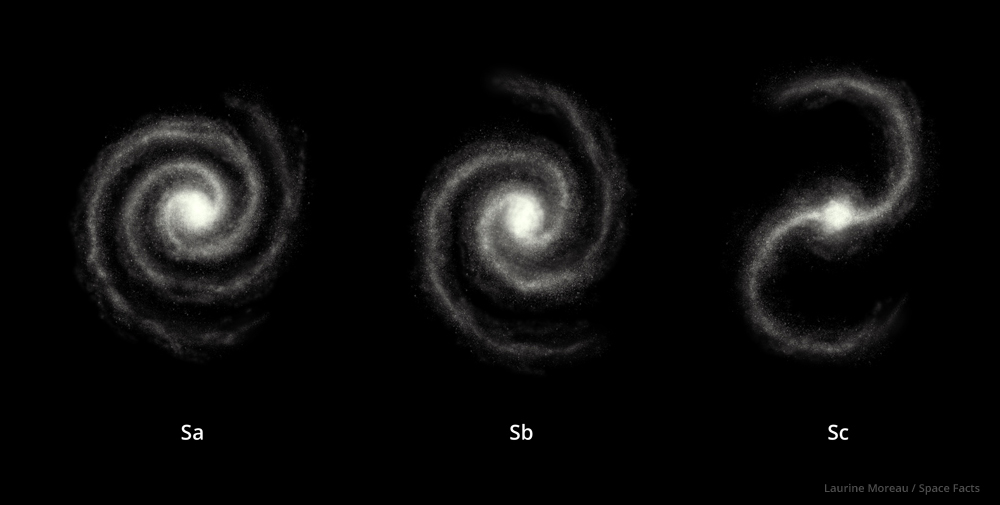
\includegraphics[scale=0.25]{galaxies/spiral/spiral-galaxies} \end{center}
			\end{itemize}
		\item $\frac{2}{3}$ spirals have an additional bar-like elongation of stars extending from the central bulge at the ends of which the spiral arms begin
			\begin{itemize}[noitemsep]
				\item the proportion of barred galaxies has changed over the history of the universe from 10\% to the current amt
				\item these are denoted by the additional label $SB$
				\begin{center} 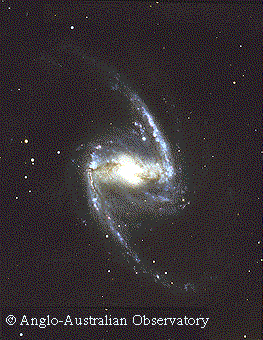
\includegraphics[scale=0.5]{galaxies/spiral/bar} \end{center}
			\end{itemize}
		\item \textbf{bulge} --- a huge, tightly packed central group of stars, often defined as the excess of stellar light above the inward extrapolation of the outer (exponential) disk light. Many bulges are thought to host a supermassive black hole at their centers.
	\end{itemize}
	\\
	\hline
	Celestial Bodies &
	\begin{itemize}[noitemsep]
		\item  The spiral arms are sites of ongoing star formation and are brighter than the surrounding disc because of the young, hot OB stars that inhabit them. Along with fully formed stars, we find sites of stellar formation, with hot glowing clouds of gas and dust forming the ``stellar nurseries" which we see as nebulae in our own galaxy.
			\begin{itemize}[noitemsep]
				\item $S_c$ spirals have the highest proportions of gas and dust, some of which is heated by stars to form nebulae
			\end{itemize}
		\item Using the Hubble classification, the bulge of $S_a$ galaxies is usually composed of Population II stars, that are old, red stars with low metal content. Further, the bulge of Sa and SBa galaxies tends to be large. In contrast, the bulges of $S_c$ and $SB_c$ galaxies are much smaller and are composed of young, blue Population I stars. Some bulges have similar properties to those of elliptical galaxies (scaled down to lower mass and luminosity); others simply appear as higher density centers of disks, with properties similar to disk galaxies.
		\item most stars are located close to the \gls{galactic plane} in conventional circular orbit around the center of the galaxy in a spheroidal bulge around the core
		\item however, some stars inhabit a \textbf{spheroidal halo/galactic spheroid}, a type of galactic halo. The orbital behavior of these stars is disputed, but they may describe retrograde and/or highly inclined orbits, or not move in regular orbits at all. Halo stars may be acquired from small galaxies which fall into and merge with the spiral galaxy.
			\begin{itemize}[noitemsep]
				\item Unlike the galactic disc, the halo seems to be free of dust, and in further contrast, stars in the galactic halo are of Population II, much older and with much lower metallicity than their Population I cousins in the galactic disc (but similar to those in the galactic bulge). The galactic halo also contains many globular clusters.
				\item The motion of halo stars does bring them through the disc on occasion, and a number of small red dwarfs close to the Sun are thought to belong to the galactic halo, and due to their irregular movement around the center of the galaxy, these stars often display unusually high proper motion.
			\end{itemize}
	\end{itemize}
	\\
	\hline
	Evolution &
	\begin{itemize}[noitemsep]
		\item the most prominent theory regarding the formation of the spiral arms is the \textbf{density wave theory} --- stars move thru intermittent periods of great density as part of their orbital cycle which form spiral shapes
			\begin{itemize}[noitemsep]
				\item the density wave rotates slower than the material in the galactic disc, so that stars and gas are able to ``overtake" the wave
				\item as interstellar gas passes thru the density wave, it becomes more dense, leading to the formation of new stars
				\item the hottest stars live for a very short time, so they appear bright within the spiral arms during their lifetime, but as they pass out of the spirals and into the galactic disk, they die and become dim, explaining the contrast in brightness
			\end{itemize}
		\item the older stars of the bulge and halo are thought to have formed through the primordial collapse of individual gas clouds early in the history of the Universe
			\begin{itemize}[noitemsep]
				\item bulges, especially those of $S_c$ and $S_d$ type galaxies, sometimes contain younger stars; after the spiral bulges of these galaxies had formed through primordial collapse, they also experienced some form of secular evolution --- through accretion processes or the actions of spiral arms or a central bar
			\end{itemize}
		\item disks are thought to form after the primordial collapse event responsible for the formation of the spheroidal bulge and halo, possibly through the cooling of the hot gas contained within the halo of the newly formed galaxy. however, spiral galaxies have both thick disks (composed entirely of stars) and thin disks (also containing cold gas).
			\begin{itemize}[noitemsep]
				\item on average, the thick disk is older than the thin disk but younger than the bulge. It has therefore been suggested that the thick disk may have formed through a significant merger event early in the Galaxy?s history. Both observations and N-body modelling indicate that such an event would disrupt the thin disk and consume a significant fraction of the cold gas in a burst of new star formation, so the proposed merger event must have taken place before the thin disk had time to fully form.
				\item An alternative to this major merger scenario is one in which the thick disk formed relatively slowly through the actions of multiple minor mergers. Once the merger events had formed the thick disk, the stars retained the scale height of the thick disk while the cold gas collapsed back into the galactic plane to form the thin disk.
				\item ongoing star formation takes place in the thin disk. This star formation is usually on the leading edge of the spiral arms where the cold gas of the thin disk is compressed.
			\end{itemize}
	\end{itemize}
	\\
	\hline
\end{longtabu}
			